% Updated by Michael Gertz, April 2021
%%%%%%%%%%%%%%%%%%%%%%%%%%%%

\documentclass{beamer}
%\usepackage[ngerman]{babel}
\usepackage[utf8]{inputenc}

\usepackage{color}
\usepackage{graphicx}
\usepackage{fancybox}
\usepackage{comment}

\usepackage{beamerthemesplit}
\usetheme[compress]{Heidelberg}
\definecolor{unirot}{rgb}{0.5976525,0,0}
\usecolortheme[named=unirot]{structure}


\title[Dense Retrieval with Entity Views]{Dense Retrieval with Entity Views}
\subtitle{Seminar ``Modern Infomation Retrieval'', Summer 2023}
%\subtitle{Subtitle}
\author[Johannes Sindlinger]{Johannes Gabriel Sindlinger}
\date{\today}
\institute[Uni HD]{
Heidelberg University\\
Institute of Computer Science\\
%Database Systems Research Group\\
\color{unirot}{johannes.sindlinger@stud.uni-heidelberg.de}}

%---------------------------------------%
%---------- RECURRING OUTLINE ----------%
% have this if you'd like a recurring outline
\AtBeginSection[]  % "Beamer, do the following at the start of every section"
{
\begin{frame}<beamer> 
\frametitle{Outline} % make a frame titled "Outline"
\tableofcontents[currentsection,hideallsubsections]  % show TOC and highlight current section
\end{frame}
}
%----------------------------------------


\begin{document}
\frame[plain]{\titlepage}
\frame{\frametitle{Outline}\tableofcontents[hideallsubsections]}

%========================================
%========================================

\section[Motivation]{What's the issue? -- Motivation}

\frame{
\frametitle{Introduction -- General Model}
\begin{figure}
  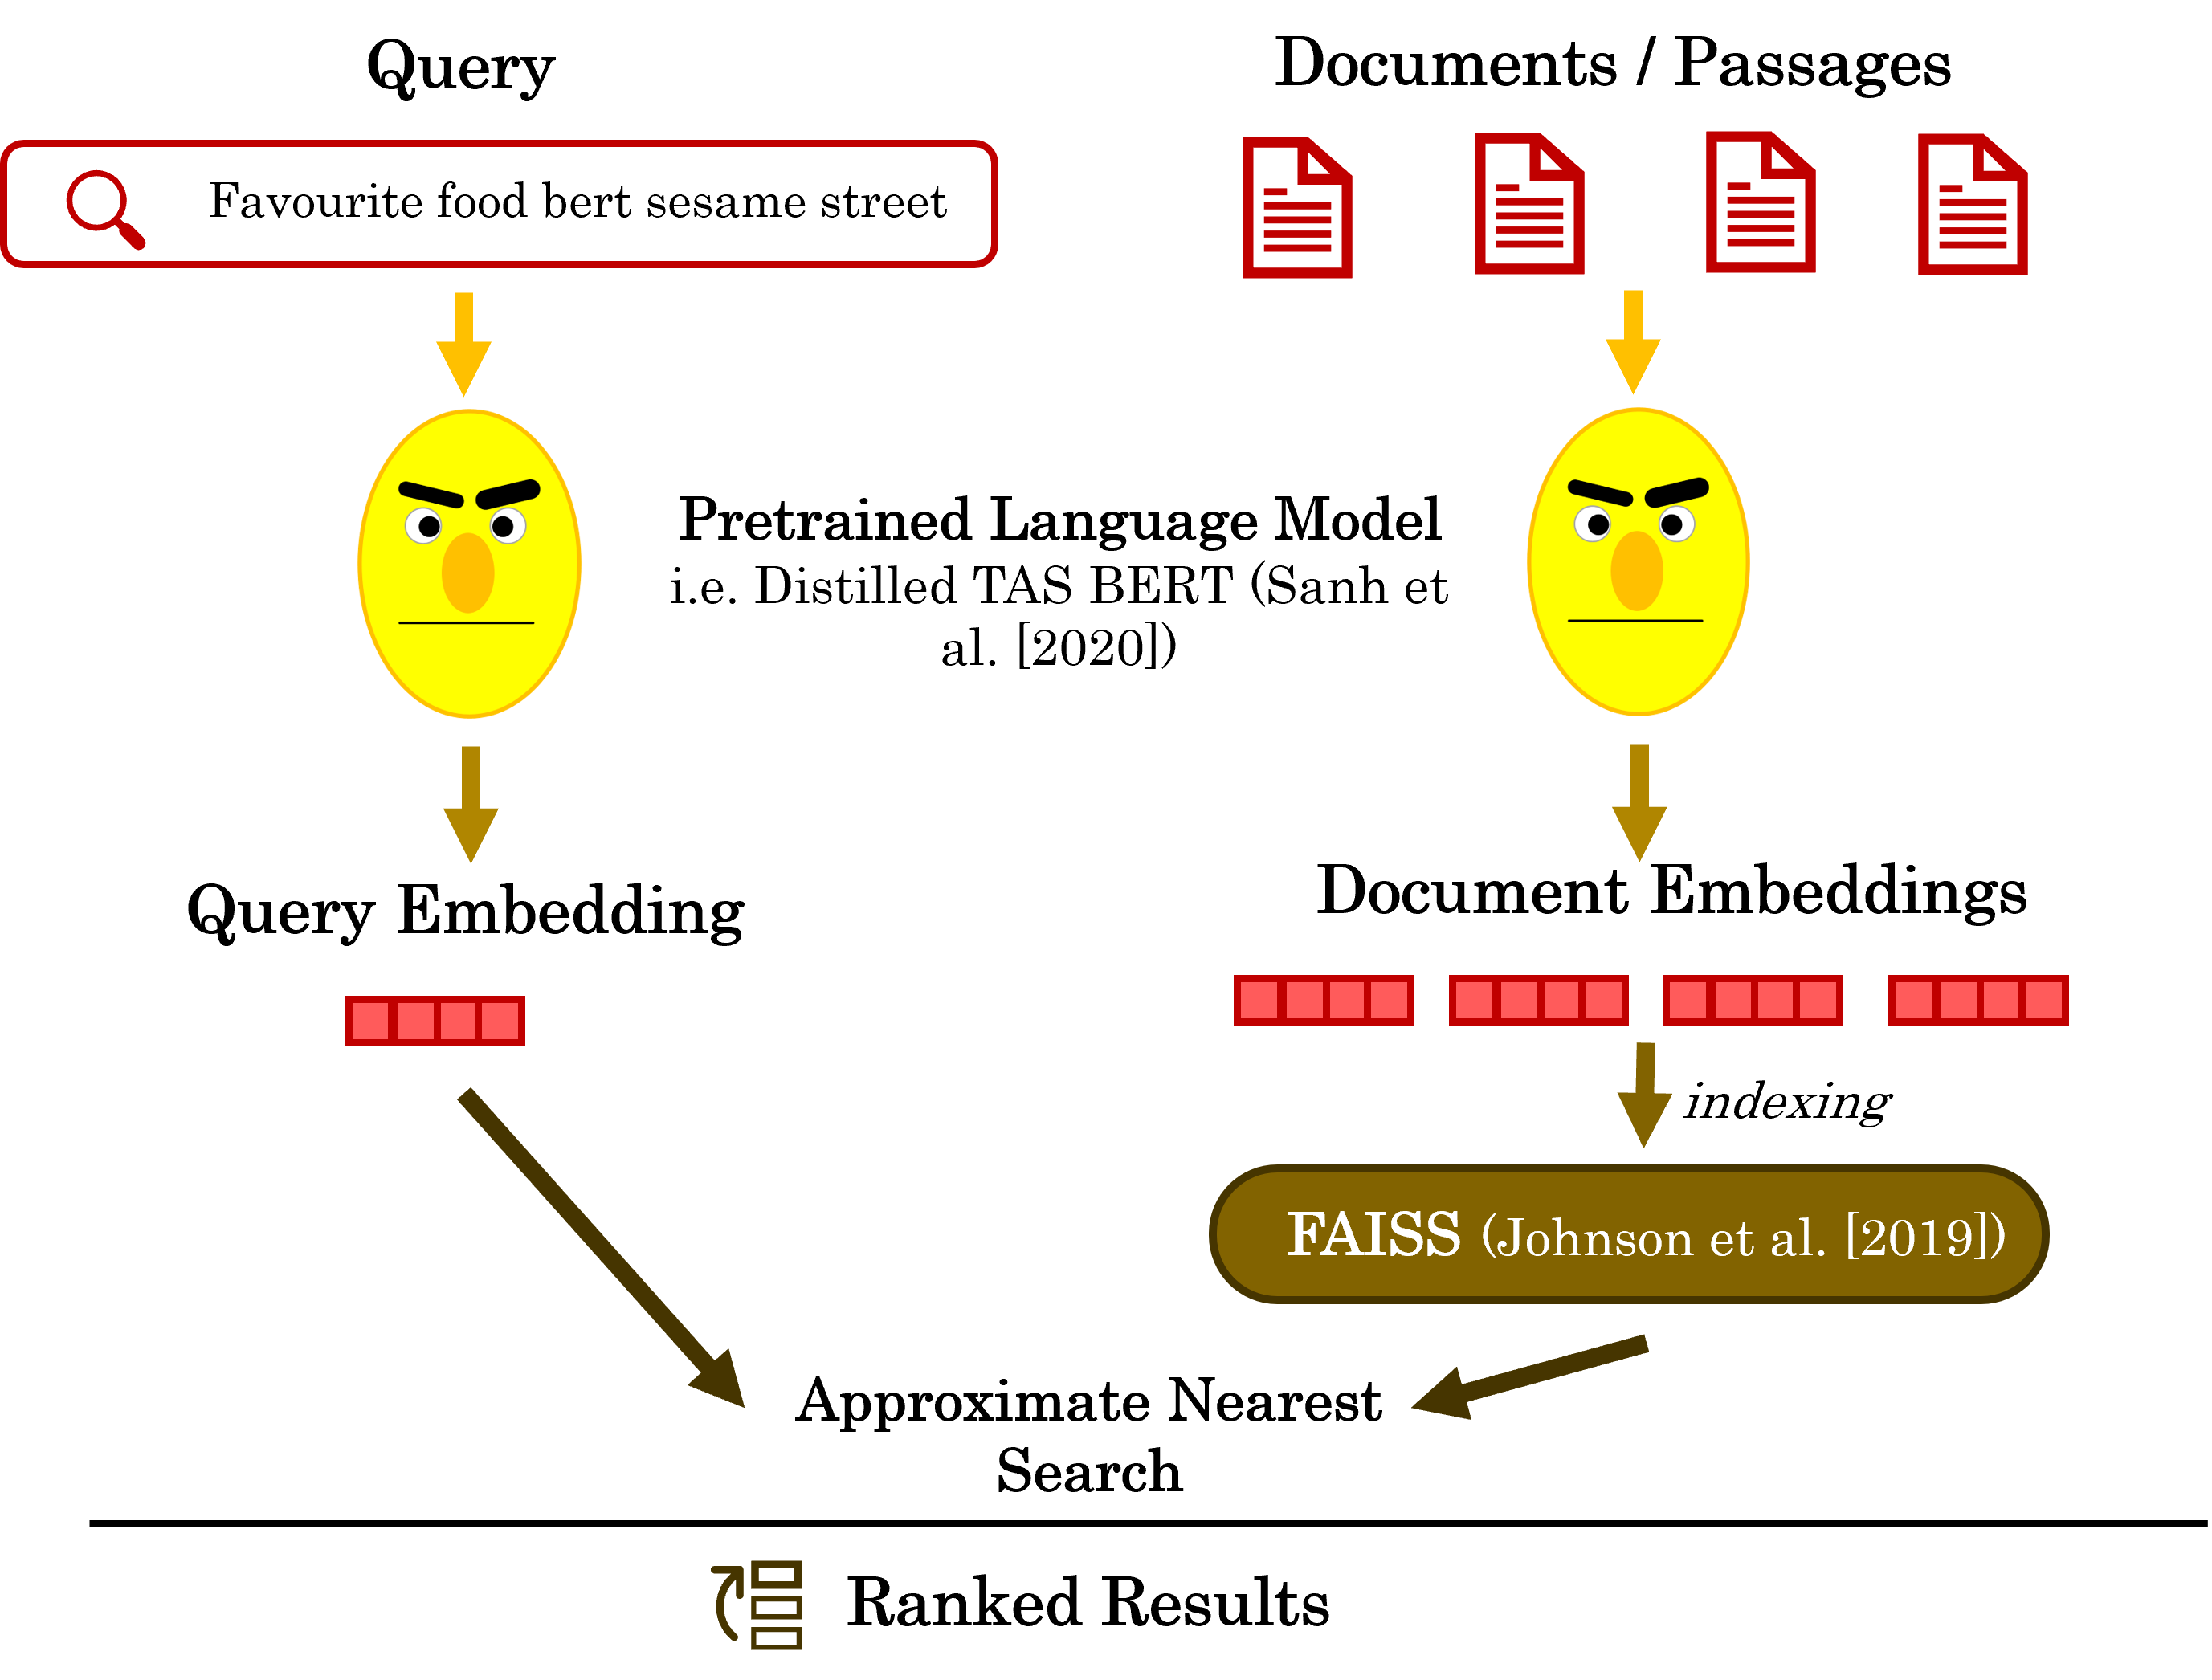
\includegraphics[width=0.85\textwidth]{Grafiken/Dense_Retrieval_Overview.png} 
\end{figure}
}

%----------------------------------------

\frame{
\frametitle{Motivation}
\begin{figure}
  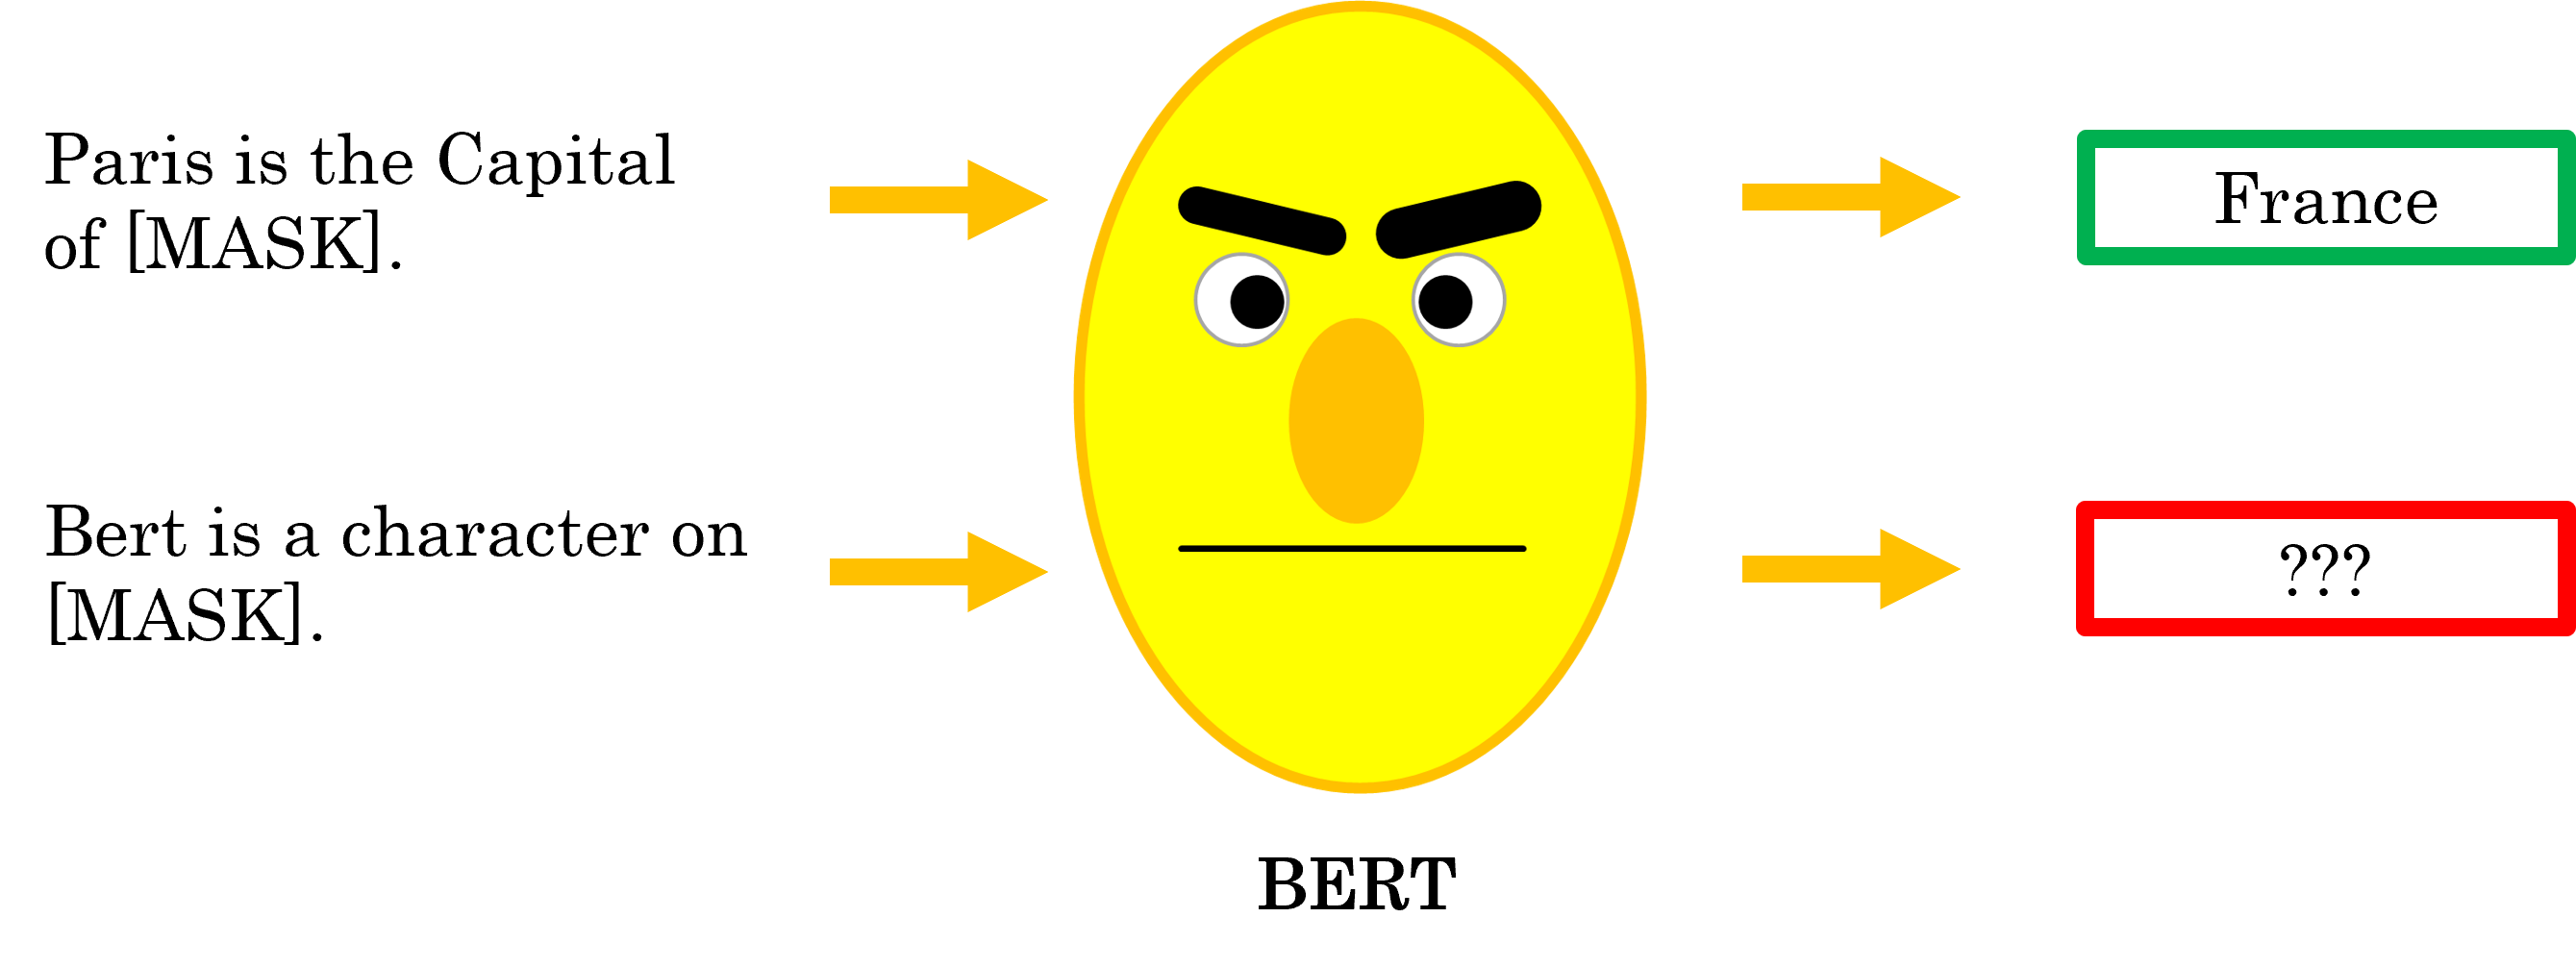
\includegraphics[width=\textwidth]{Grafiken/Problem.png} 
\end{figure}
$\Rightarrow$ Language models do not fully capture information about real-world entities, especially for uncommon entities.
}

\frame{
\frametitle{Example}
\begin{figure}
  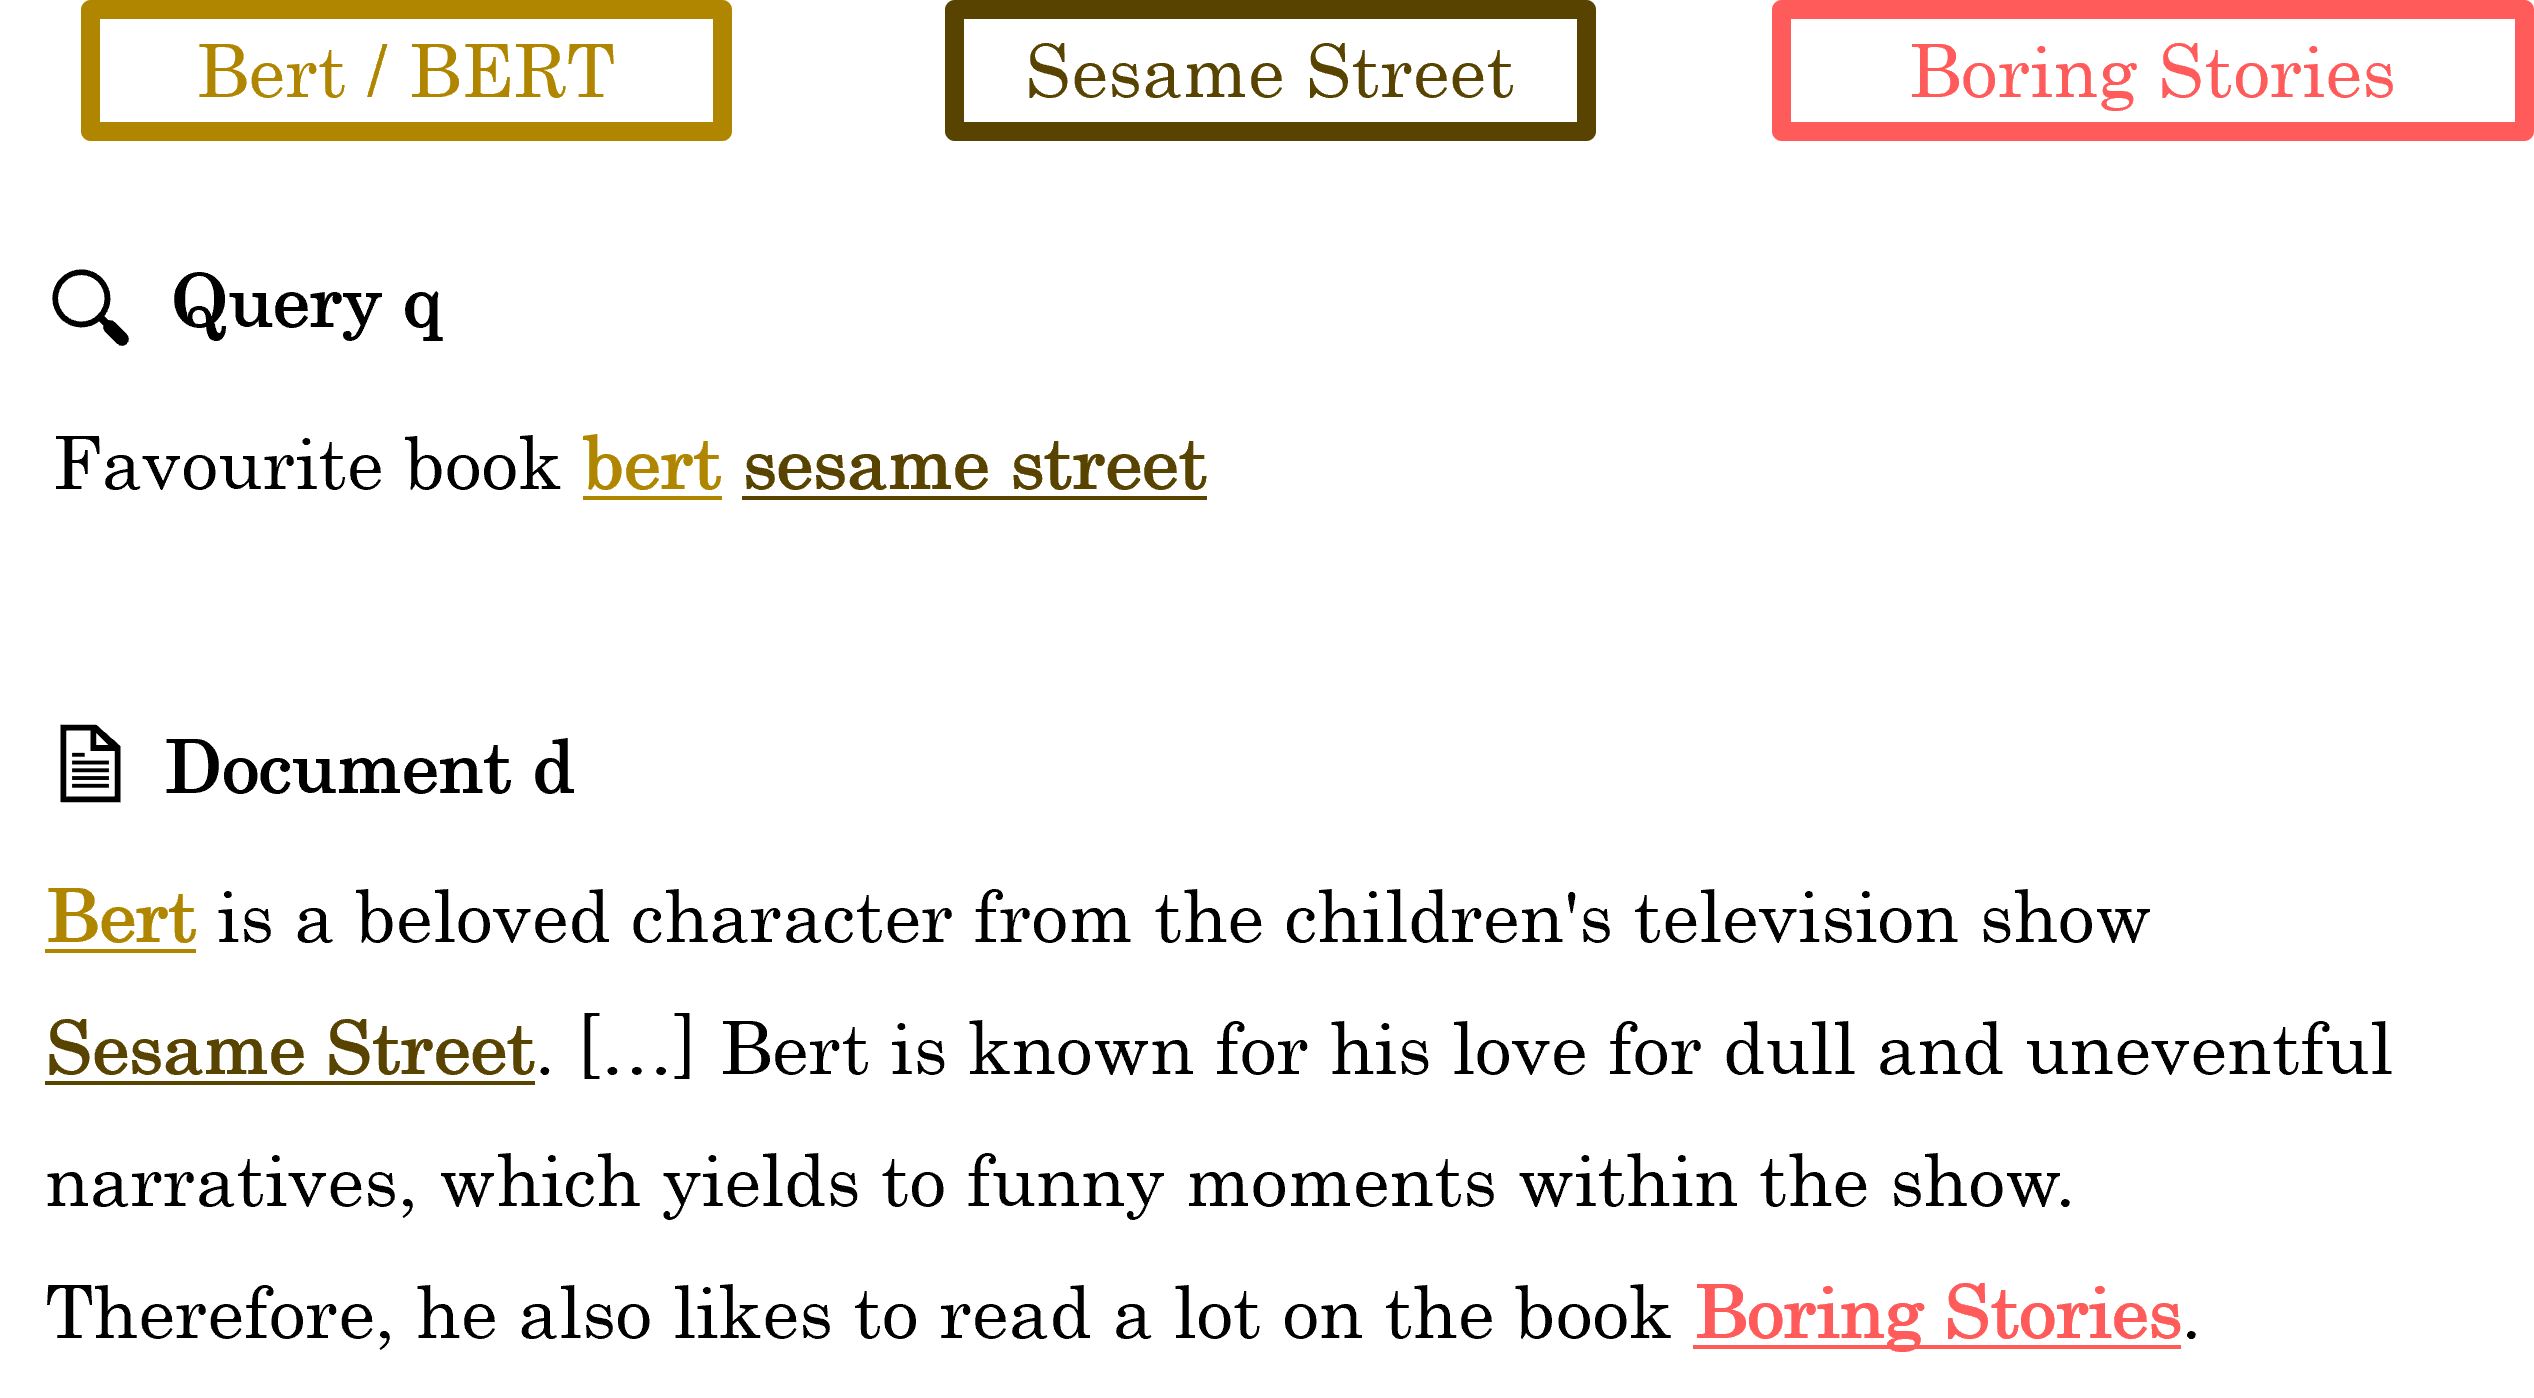
\includegraphics[width=0.88\textwidth]{Grafiken/Example_3_Entities.png} 
\end{figure}
}


%---------------------------------------
%---------------------------------------
\section[Related Work]{What has been already there? – Related Work}

\frame{
\frametitle{Related Work}
TODO
}

%---------------------------------------
%---------------------------------------
\section[Methodology]{What‘s new? – Methodology}

\frame{
\frametitle{General Model}
\begin{figure}
  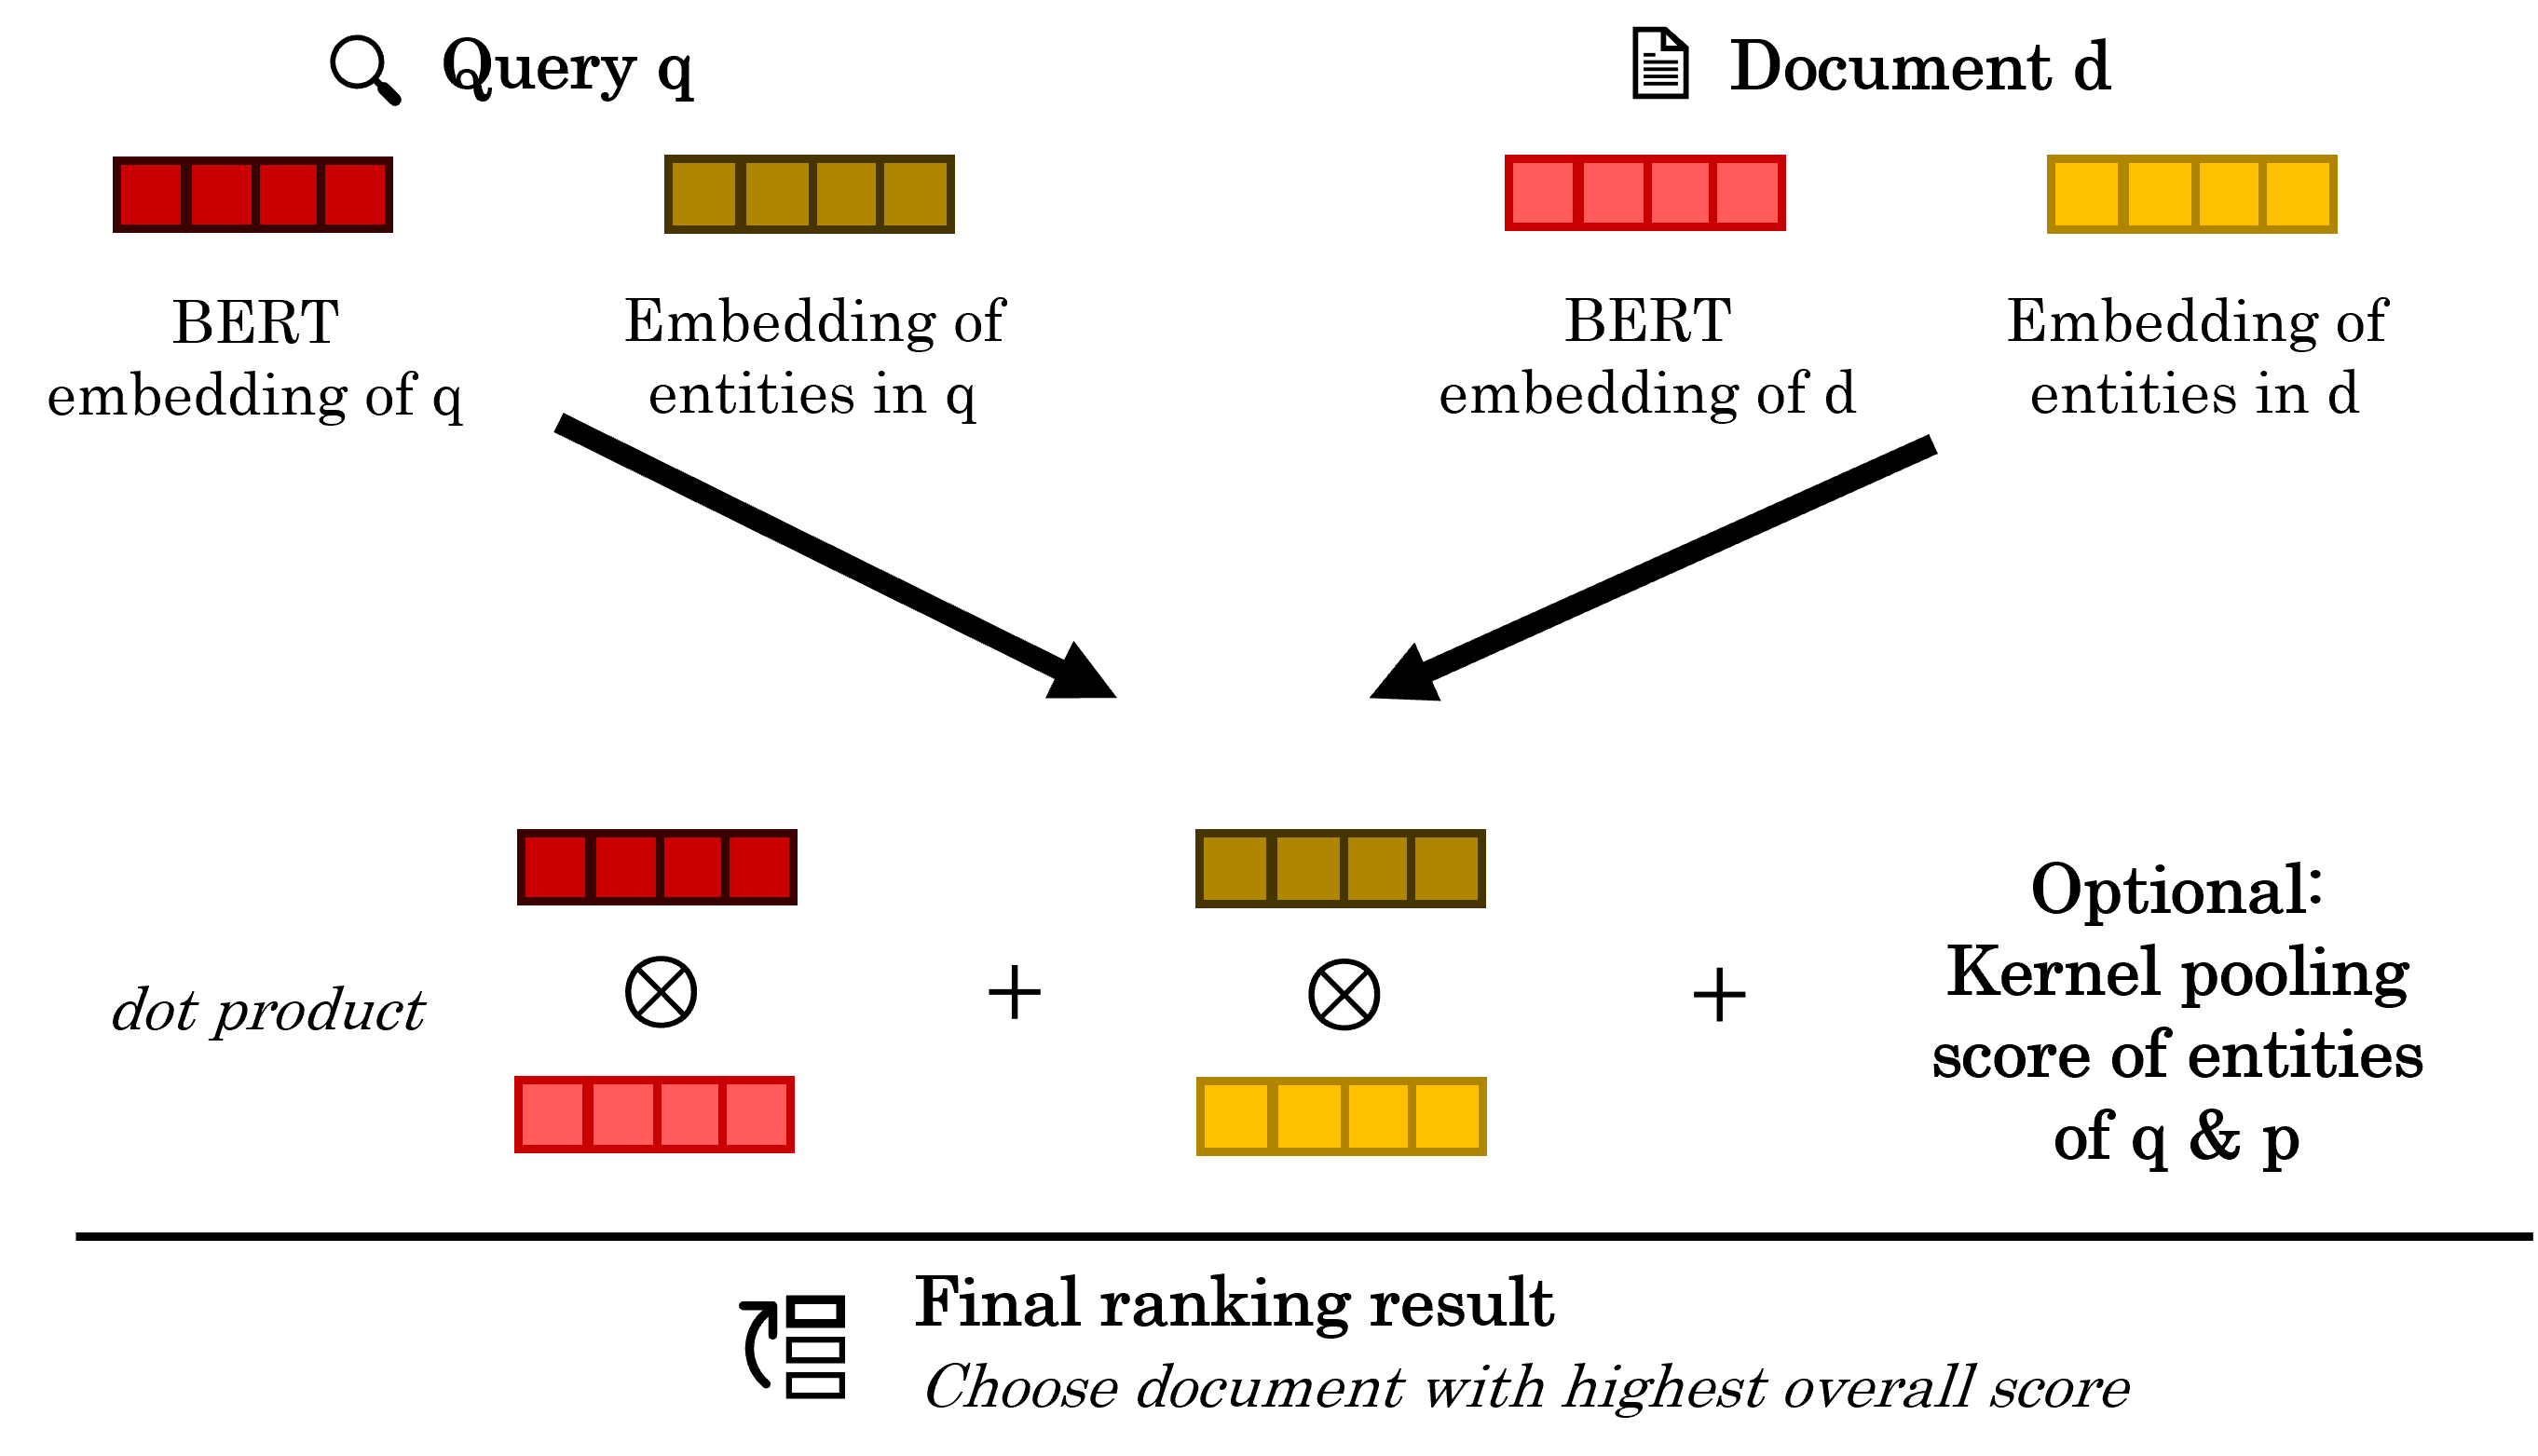
\includegraphics[width=\textwidth]{Grafiken/Main_Idea.png} 
\end{figure}
}

\frame{
\frametitle{Extracting Entities}
\begin{figure}
  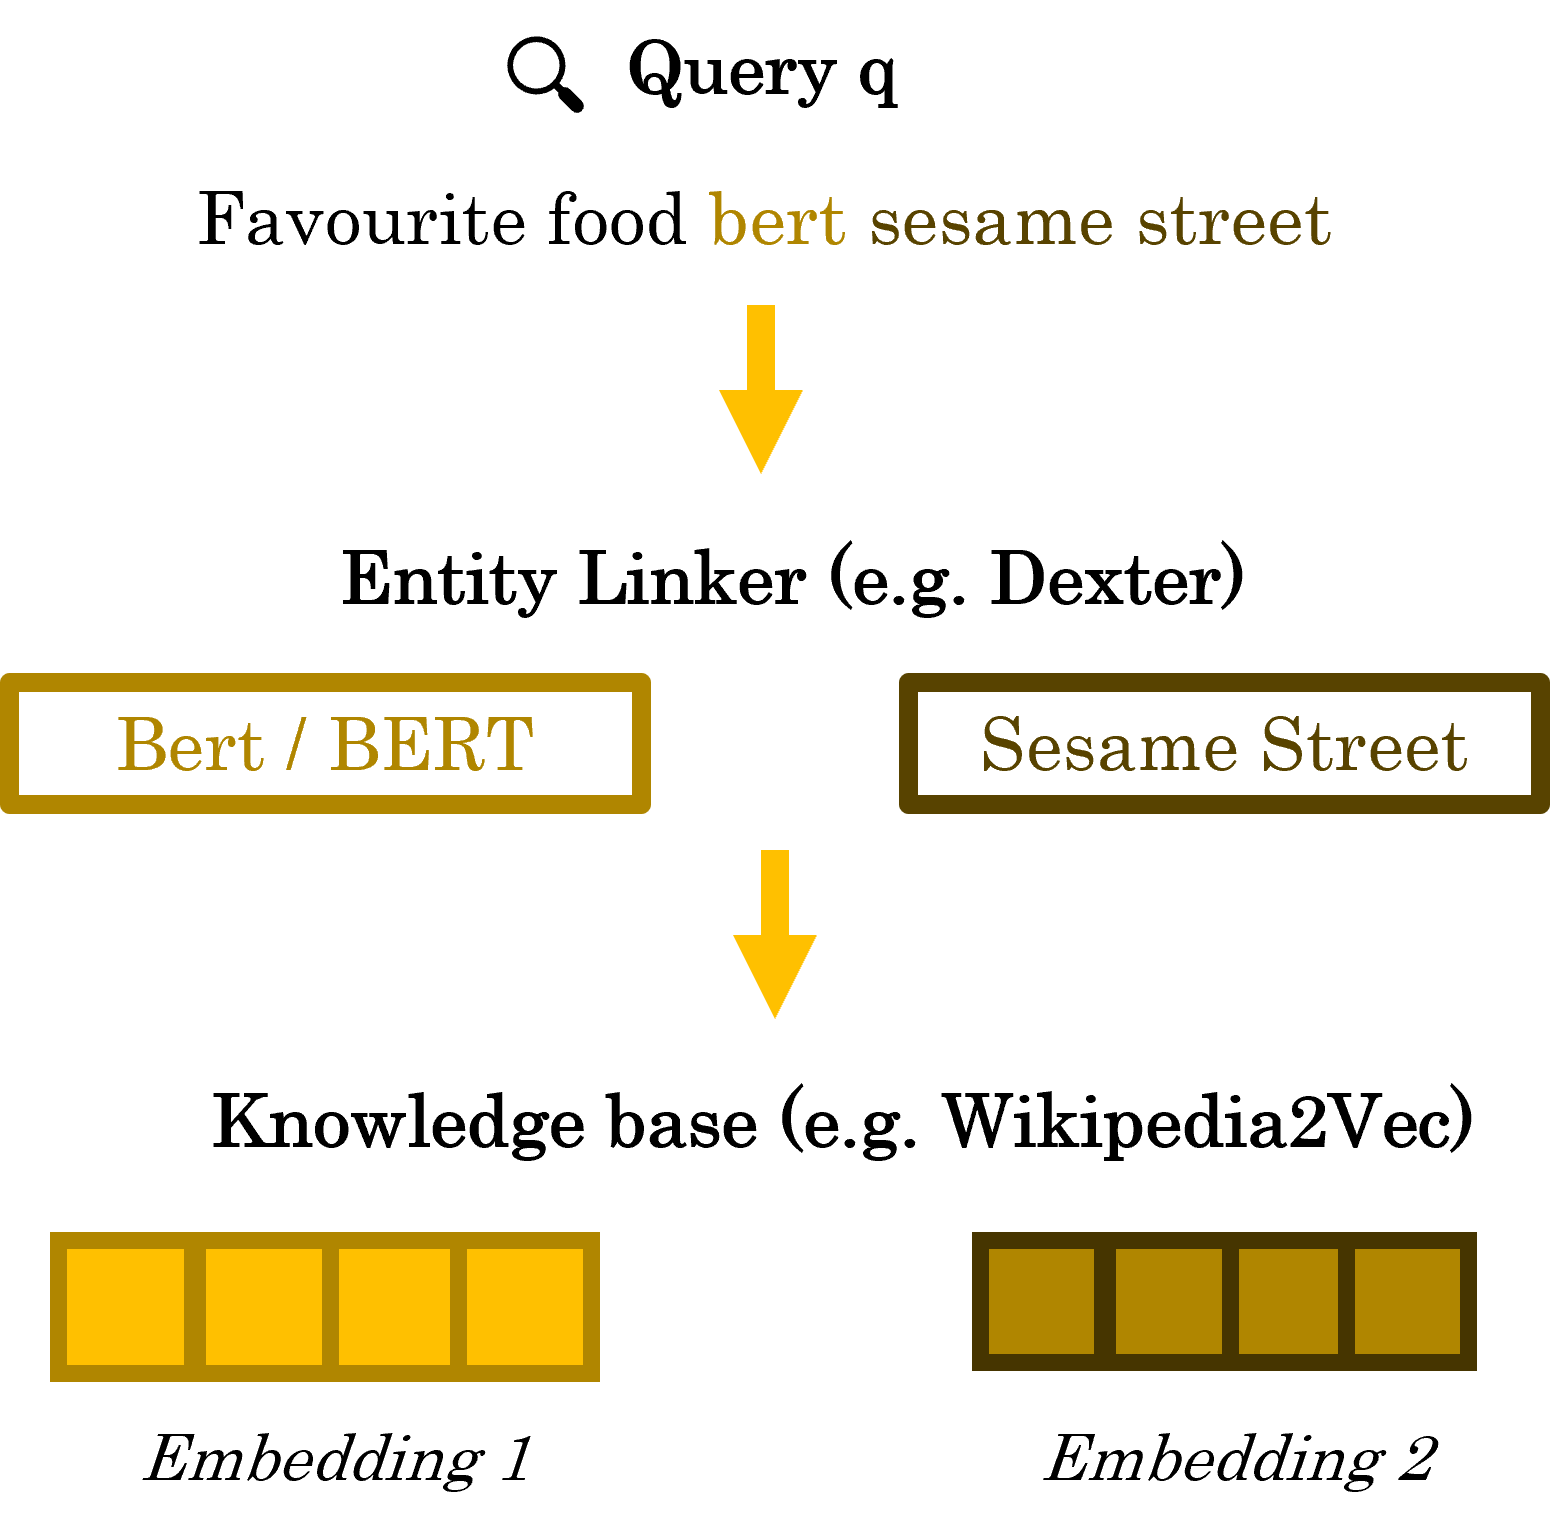
\includegraphics[width=0.57\textwidth]{Grafiken/Extracting_Entities.png} 
\end{figure}
}


\frame{
\frametitle{Multiple Approaches}
\begin{itemize}
  \item Single Entity Representation (EVA Single)
  \item Query-Aware Single Entity Representation (EVA Single-QA)
  \item Multiple Entity View Representation (EVA Multi)
\end{itemize}
\vspace{0.5cm}
$\Rightarrow$ Optionally for all models: Adding Kernel pooling score (e.g. KNRM)
}

\frame{
\frametitle{Single Entity Representation}
\begin{itemize}
  \item Same method for queries and documents
  \item For queries: Method is applied to all three approaches
\end{itemize}
\begin{figure}
  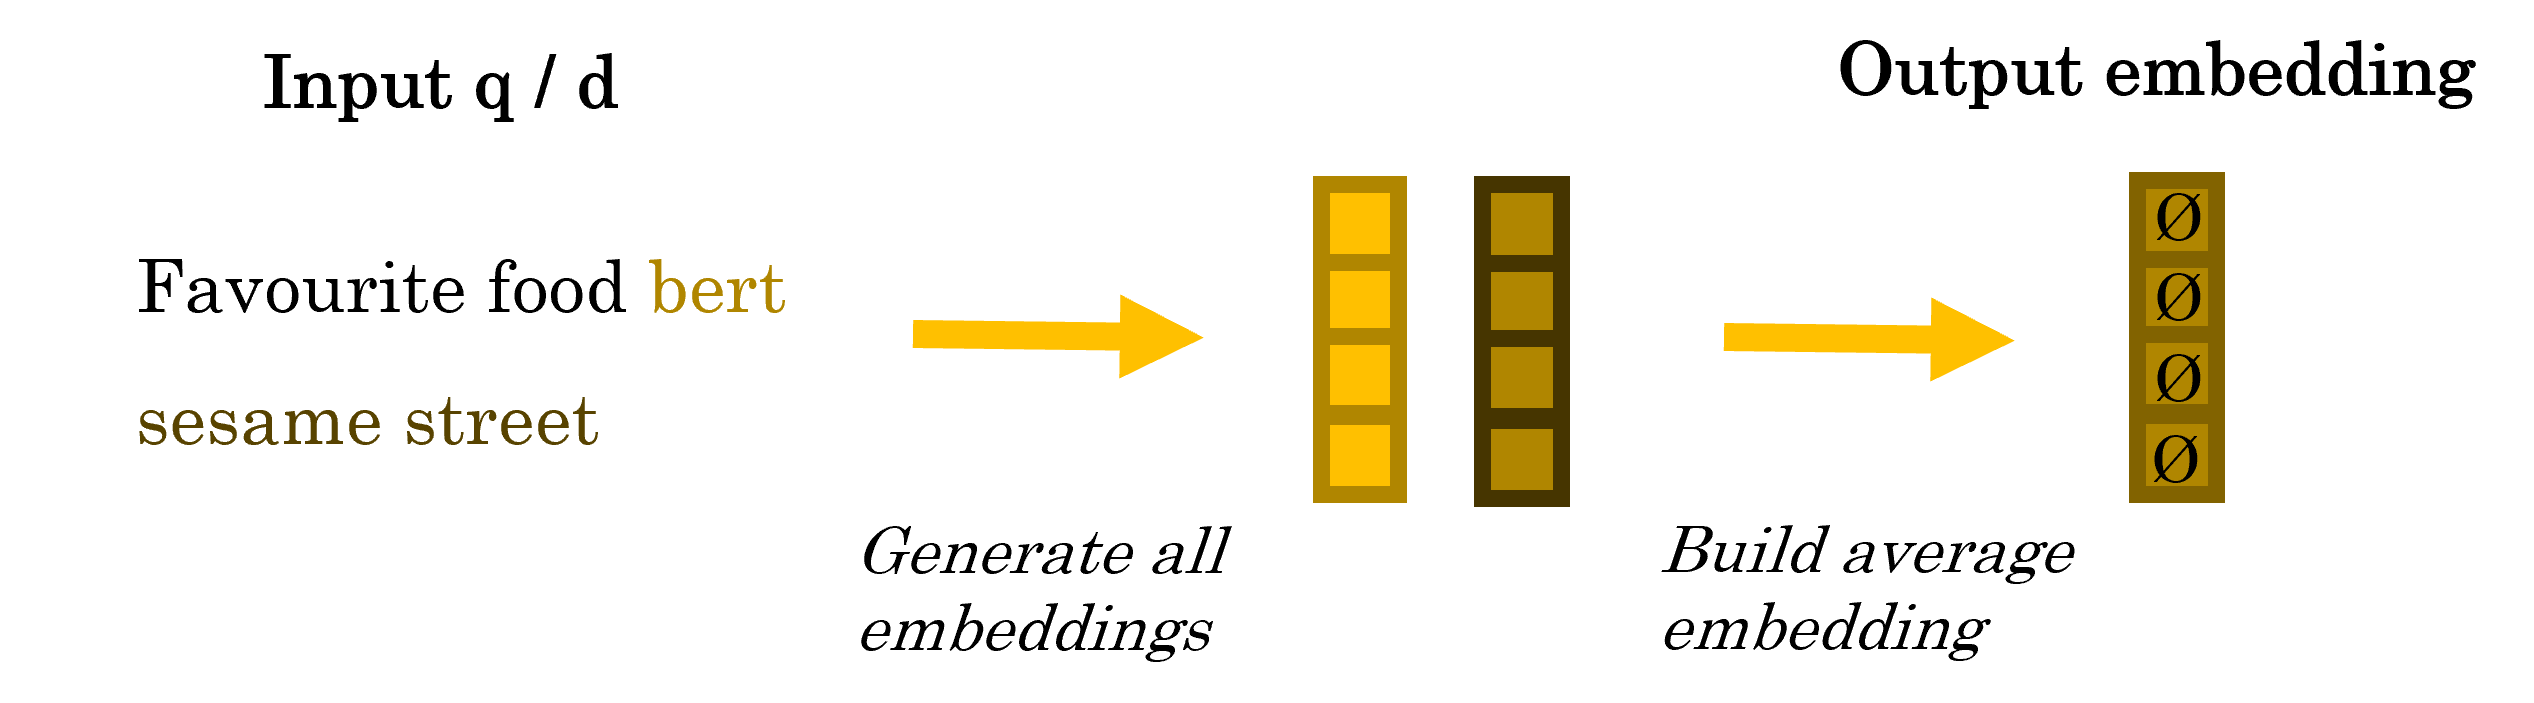
\includegraphics[width=\textwidth]{Grafiken/Single_Entity_Representation.png} 
\end{figure}
$\Rightarrow$ Problem: No focus on query information, possibly including irrelevant entities
}

\frame{
\frametitle{Query-Aware Single Entity Representation}
\begin{itemize}
  \item Assumption: Query is known before calculations
  \item Idea: Select only entities in document with high similarity to query entities
\end{itemize}
\begin{figure}
  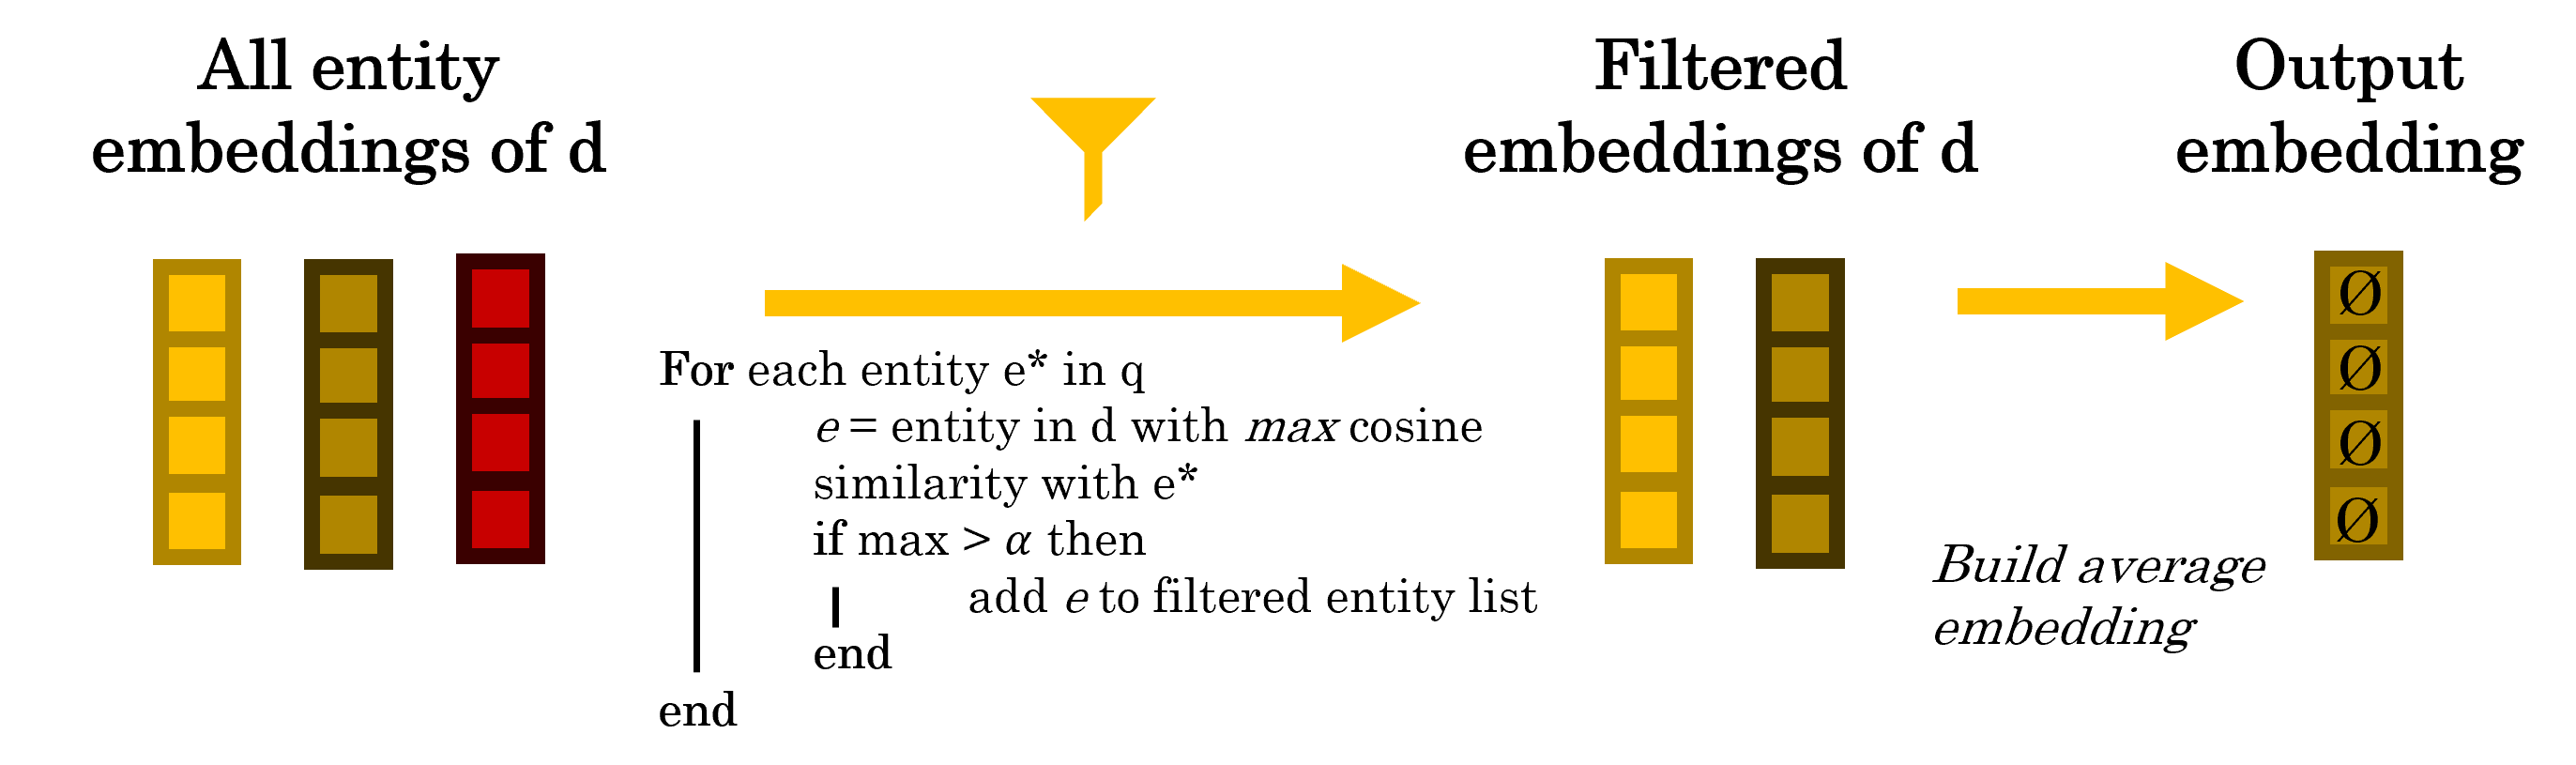
\includegraphics[width=\textwidth]{Grafiken/QA_Single_Entity_Representation.png} 
\end{figure}
Due to ???, output embeddings are transformed using a learned Matrix $W_{\text{entity}}$. 
$\Rightarrow$ Embedding$_{\text{final}} = \text{Embedding}_{\text{Output}}^T W_{\text{entity}}$.
}


\section[Evaluation \& Results]{What‘s the outcome? –- Evaluation \& Results
}






\end{document}
